\documentclass[a4paper]{article}
\usepackage{tikz}
\usetikzlibrary{matrix,fit}

\begin{document}
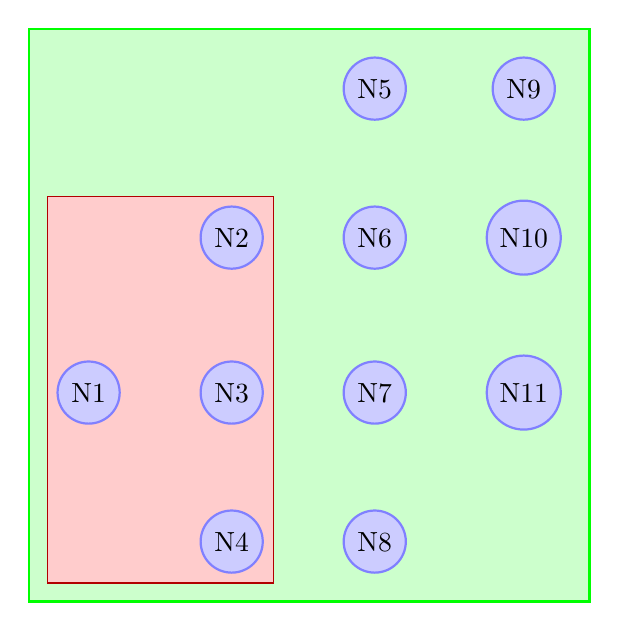
\begin{tikzpicture}[
   inner/.style={circle,draw=blue!50,fill=blue!20,thick,inner sep=3pt},
   outer/.style={draw=green,fill=green!20,thick,inner sep=10pt, column sep=1cm, row sep=1cm}
]
  \matrix (A) [matrix of nodes,outer, nodes={inner,draw}]{
       &    & N5 & N9  \\
       & N2 & N6 & N10 \\
     N1 & N3 & N7 & N11 \\
       & N4 & N8 &     \\
   };   
\node[draw=red!70!black,fill=red!20,fit={(A-3-1) (A-2-2) (A-4-2)}] {};
\foreach \Pos/\Nodo in {A-3-1/N1,A-2-2/N2,A-3-2/N3,A-4-2/N4}
  \node[inner] at (\Pos) {\Nodo};
\end{tikzpicture}

\end{document}
